\chapter{Results and Discussion}
\label{ch:results}

\section{Overview}

This chapter reports the end-to-end results: pruning, constraint pressure,
assignment, amortisation, scaling, and trust and fault behaviour; the solver
results were given in Chapters~\ref{ch:solvers} and~\ref{ch:exact}. Negative
results are reported with the same prominence as positive ones, because they
define where the architecture should and should not be used.
Table~\ref{tab:res:scoreboard} gives the whole picture.

\begin{table}[htbp]
\centering
\caption{Scoreboard of the main quantitative results.}
\label{tab:res:scoreboard}
\small
\begin{tabularx}{\linewidth}{@{}X l@{}}
\toprule
Measurement & Result \\
\midrule
Encoding agreement with independent re-derivation & within $2.3\times10^{-10}$ \\
Exact-solve rate of four annealing samplers & 48 to 64\% \\
Projected annealer: small instances / against MILP & 100\% / 95\% exact \\
MILP against projected annealer, time & about 100 times faster \\
Trust-aware GNN against trust-only & $+8.1$ pts, CI $[+4.2,+11.7]$, $p=0.016$ \\
Trust-aware GNN against random / no-graph & $+13.8$ pts / $+1.7$ pts (n.s.) \\
QUBO pruner against best repaired baseline & $-0.1$ to $-4.1$ pts, never ahead \\
QUBO degree violations at any pressure & zero \\
Cloud-trained readout against fixed weights & $-3.9$ pts (n.s.) \\
Recovery after an injected fault & 3 to 4 cycles \\
\bottomrule
\end{tabularx}
\end{table}

\section{The Pruner Comparison}

Table~\ref{tab:res:pruners} compares the six pruners on identical scenarios of
10 rovers, 20 cycles and 16 seeds with drifting reliability, at the project's
original fixed budget of $K=15$ units.

\begin{table}[htbp]
\centering
\caption[Pruner comparison, 10 rovers, 20 cycles, 16 seeds, fixed budget $K=15$.]{Pruner comparison, 10 rovers, 20 cycles, 16 seeds, fixed budget
$K=15$. Violations are mean counts per run (degree / budget / connectivity).
$^{\dagger}$See Section~\ref{sec:res:audit}.}
\label{tab:res:pruners}
\footnotesize
\setlength{\tabcolsep}{4pt}
\begin{tabular}{@{}l r r r r r r r@{}}
\toprule
Pruner & Success & Offload & Del.\ fail & Solve & Spearman & AUC & Violations \\
\midrule
full graph & 36.0\% & 1.000 & 0.385 & none & 0.271 & 0.683 & 158.8 / 20.0 / 0.4 \\
threshold & 37.0\% & 0.955 & 0.340 & $<0.01$~ms & 0.254 & 0.624 & 131.7 / 20.0 / 2.3 \\
top-$K$ & 36.4\% & 0.898 & 0.309 & $<0.01$~ms & 0.251 & 0.683 & 53.6 / 20.0 / 10.0 \\
threshold+repair & 34.3\% & 1.000 & 0.396 & 0.4~ms & 0.249 & 0.640 & 4.7 / 20.0 / 0.4 \\
top-$K$+repair & 34.8\% & 1.000 & 0.392 & 0.2~ms & 0.242 & 0.638 & 3.4 / 19.9 / 0.4 \\
QUBO (ours) & 32.2\% & 0.998 & 0.418 & 1435~ms & 0.272 & 0.669 & 0.0 / 19.9$^{\dagger}$ / 0.4 \\
\bottomrule
\end{tabular}
\end{table}

\subsection{The Audit Caught the Audit}
\label{sec:res:audit}

The relaxation bookkeeping of Section~\ref{sec:sol:ladder} exposed a problem
in the project's own earlier results. At $K=15$ the production pruner used the
\emph{no-budget} rung in 319 of 320 cycles: at ten rovers a budget of 15 units
is below the cost of any connected subgraph, so the ladder dropped it, and the
QUBO row of every earlier pruner table was in effect unconstrained. This is
precisely what the bookkeeping was built to catch, and an argument for always
logging relaxations rather than asserting feasibility. All
constraint-relevant conclusions were re-run at a budget that is both binding
and feasible, $K=0.75\times$ the full-graph cost, where the QUBO solved with
every constraint in 320 of 320 cycles (Fig.~\ref{fig:res:binding}).

\begin{figure}[htbp]
\centering
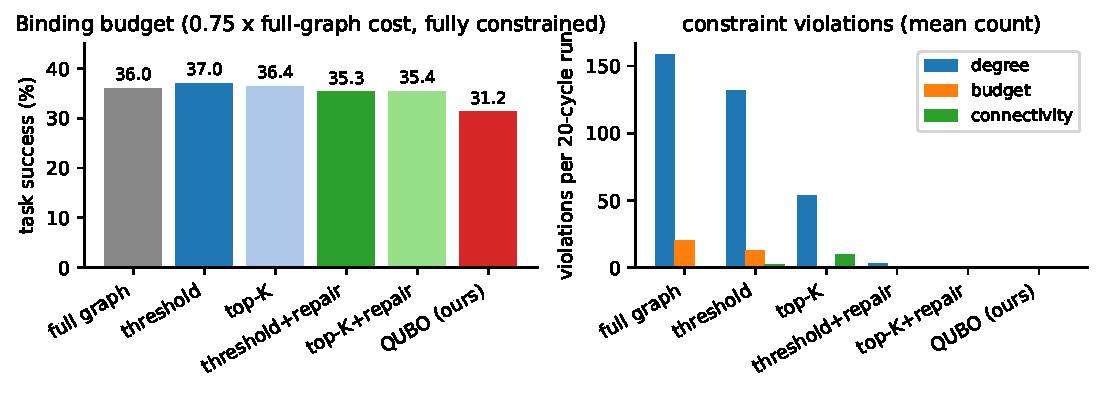
\includegraphics[width=0.95\linewidth]{figures/fig_bench_binding.pdf}
\caption{Mission success and constraint violations of the six pruners at a
binding, feasible budget ($0.75\times$ the full-graph cost).}
\label{fig:res:binding}
\end{figure}

\subsection{What the Guarantees Cost and Buy}

At the binding budget the QUBO pruner is behind on raw success by 4.1 points
against threshold+repair (95\% CI $[-6.4,-1.9]$, $p=0.004$), by 4.2 points
against top-$K$+repair (CI $[-7.0,-1.5]$, $p=0.017$) and by 5.7 points against
the constraint-blind threshold pruner ($p=0.002$). Comparing only against
constraint-blind pruners had overstated the cost of the guarantees by about two
points, but the corrected gap remains significant. What the QUBO buys is the
guarantee itself: it is the only arm with zero violations (the repaired
baselines leave 1.1 to 3.1 degree and 0.8 to 0.9 connectivity violations per
run),
and it has the best trust Spearman (0.295 against 0.251 to 0.271), though not
the best AUC. The delivery metrics show its weakness (Fig.~\ref{fig:res:delivery}):
a delivery-failure rate 4.4 points worse than threshold+repair (CI
$[+1.4,+8.0]$) and 11.8 points worse than top-$K$, and a recall of
delivery-critical links of 0.67, against 0.82 for the repaired baselines and
0.93 for the threshold pruner; only the constraint-blind top-$K$, which keeps
half of the links, is lower (0.56). The edge-local utility
ranks links by their own quality rather than by how much delivery depends on
them, so the optimum sometimes prunes exactly the redundancy that bottleneck
paths need.

\begin{figure}[htbp]
\centering
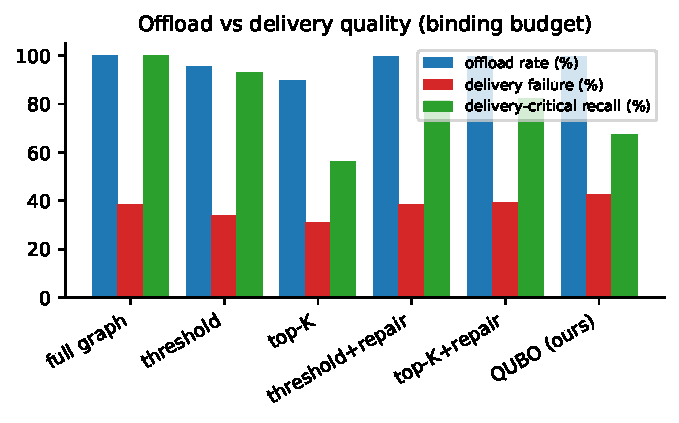
\includegraphics[width=0.72\linewidth]{figures/fig_delivery.pdf}
\caption{Offload rate, delivery-failure rate and delivery-critical recall of
each pruner at the binding budget.}
\label{fig:res:delivery}
\end{figure}

\section{Constraint Pressure}
\label{sec:res:pressure}

Does the guarantee ever turn into a success advantage when constraints bite
hard? Table~\ref{tab:res:pressure} and Fig.~\ref{fig:res:budget} answer it.

\begin{table}[htbp]
\centering
\caption{Constraint-pressure sweep, 10 rovers, 20 cycles, 16 seeds per cell;
differences in percentage points with permutation $p$-values.}
\label{tab:res:pressure}
\footnotesize
\setlength{\tabcolsep}{4pt}
\begin{tabular}{@{}l r r r r@{}}
\toprule
Constraint & Level & QUBO & Best repaired & QUBO $-$ best \\
\midrule
budget $\beta_K$ & 0.35 & 34.6\% & 34.7\% & $-0.1$ ($p=1.00$) \\
 & 0.50 & 31.6\% & 35.2\% & $-3.7$ ($p=0.033$) \\
 & 0.75 & 31.3\% & 35.4\% & $-4.1$ ($p=0.004$) \\
 & 1.00 & 31.7\% & 35.3\% & $-3.7$ ($p=0.020$) \\
degree $D$ & 2 & 30.9\% & 34.3\% & $-3.3$ ($p=0.15$) \\
 & 3 & 32.2\% & 34.3\% & $-2.1$ ($p=0.10$) \\
 & 4 & 33.3\% & 34.8\% & $-0.9$ ($p=0.52$) \\
roster $|R|$ & 3 & 32.2\% & 34.3\% & $-2.1$ ($p=0.10$) \\
 & 5 & 32.4\% & 35.1\% & $-2.7$ ($p=0.058$) \\
 & 8 & 34.6\% & 37.8\% & $-3.2$ ($p=0.020$) \\
\bottomrule
\end{tabular}
\end{table}

\begin{figure}[htbp]
\centering
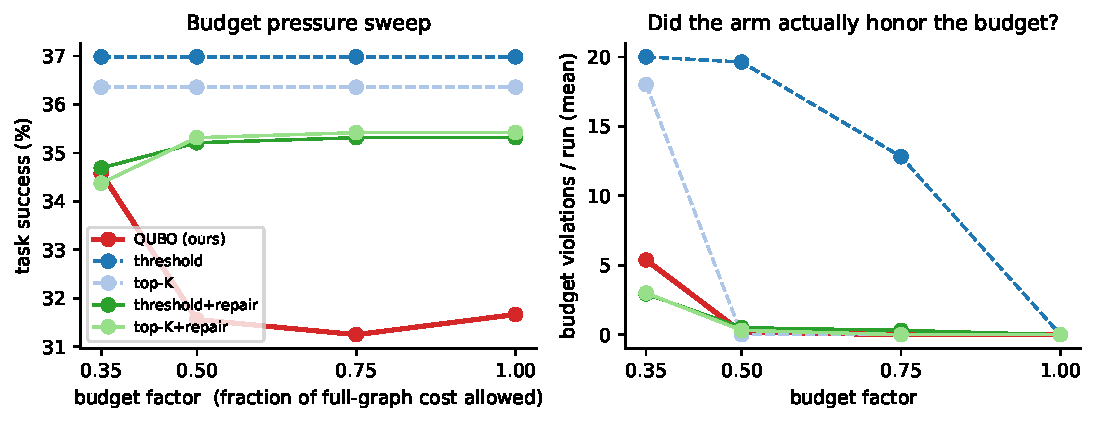
\includegraphics[width=0.95\linewidth]{figures/fig_budget_sweep.pdf}
\caption{Budget pressure sweep: success by arm (left) and whether each arm
honoured the budget (right).}
\label{fig:res:budget}
\end{figure}

The answer is not the one the guarantee story predicts. At extreme budget
pressure ($\beta_K=0.35$) the QUBO ties the best repaired baseline, where even
the repaired arms cannot fully meet the budget. At every looser setting it is
behind by 2 to 4 points, and in the degree and roster sweeps the gap narrows
only as the constraint relaxes. There is no crossover, even where the
constraint-blind threshold pruner breaks the budget in 20 of 20 cycles and, at
$D=2$, exceeds degree caps 165 times per run. What holds at every level is the
guarantee: zero degree violations, budget residuals only where the budget is
infeasible (and then reported), and connectivity misses only where no pruner
could connect the roster. The guarantees are worth their cost when violating a
constraint is disqualifying (regulatory, safety or contractual), not when
success is the only currency.

\section{Assignment Ablation}

Table~\ref{tab:res:ablation} isolates the assignment stage on identical
scenarios. The trust-aware GNN beats trust-only by 8.1 points with an interval
that excludes zero and a significant permutation test, and beats random by
13.8 points. Its margin over the no-graph readout is positive but not
significant: at ten-rover density most of the value lies in the trust model,
the gates and delivery awareness, and message passing adds a small extra that
this sample cannot separate from noise.

\begin{table}[htbp]
\centering
\caption{Ablation of the assignment stage with 10 rovers, 20 cycles and 8
seeds. Differences are computed per seed, in pairs.}
\label{tab:res:ablation}
\small
\begin{tabular}{@{}l r l@{}}
\toprule
Policy & Success & Difference to the GNN \\
\midrule
random & 26.0\% & $+13.8$ pts \\
trust-only & 31.7\% & $+8.1$ pts, CI $[+4.2,+11.7]$, $p=0.016$ \\
no-graph readout & 38.1\% & $+1.7$ pts, CI $[-2.1,+6.9]$, $p=0.736$ \\
trust-aware GNN (ours) & 39.8\% & \\
\bottomrule
\end{tabular}
\end{table}

\section{Amortisation and Scaling}
\label{sec:res:staleness}

A solve of more than a second cannot run synchronously on the fog device, so
the cloud can solve every $k$ cycles while the fog device reuses the last
decision, intersected with the live graph (Table~\ref{tab:res:staleness}).
Using a decision that is two cycles old costs less than one point of success
and cuts the number of solves in half. For $k\ge4$ the differences between
seeds are larger than the effect we are trying to measure, so we report the
numbers as they are instead of drawing a smooth curve through them.

\begin{table}[htbp]
\centering
\caption{Solving in the cloud every $k$ cycles, with 10 rovers, 20 cycles and 6 seeds.}
\label{tab:res:staleness}
\small
\begin{tabular}{@{}r r r r@{}}
\toprule
Solve interval $k$ & Success & Solves per cycle & Amortised solve (ms) \\
\midrule
1 & 30.3\% & 1.00 & 1279 \\
2 & 29.4\% & 0.50 & 618 \\
4 & 26.9\% & 0.25 & 273 \\
8 & 31.9\% & 0.15 & 151 \\
\bottomrule
\end{tabular}
\end{table}

Figure~\ref{fig:res:latency} puts the time spent on pruning next to the time
spent on inference. Solving takes about five orders of magnitude longer. At
these small fleet sizes, then, the reason to prune is the guarantees it gives
and not any saving in time. It also means the solve should run in the cloud or
only every few cycles, which is what the three-tier design planned for.

\begin{figure}[htbp]
\centering
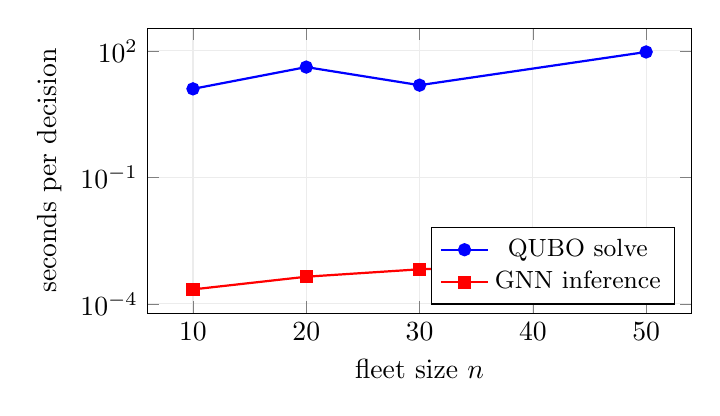
\begin{tikzpicture}
\begin{axis}[
  width=0.7\linewidth, height=5.2cm,
  xlabel={fleet size $n$}, ylabel={seconds per decision},
  ymode=log, log basis y=10,
  legend pos=south east, legend style={font=\small},
  grid=both, grid style={gray!15},
]
\addplot[mark=*, thick, blue] coordinates {(10,12.6) (20,41.4) (30,15.4) (50,94.5)};
\addlegendentry{QUBO solve}
\addplot[mark=square*, thick, red] coordinates {(10,0.00022) (20,0.00044) (30,0.00066) (50,0.00103)};
\addlegendentry{GNN inference}
\end{axis}
\end{tikzpicture}
\caption{Wall-clock time for each decision on the scaling instances. The
time drops at $n=30$ because connectivity is no longer enforced above 20
rovers.}
\label{fig:res:latency}
\end{figure}

\section{Trust Quality, Training and Faults}

The learned trust values follow the hidden reliability with a Spearman
correlation between 0.24 and 0.30 and an AUC between 0.62 and 0.68. Comparing
trust quality across pruners is not fair, because each pruner produces its own
set of outcomes, and we point this out instead of leaving it unsaid. As
reported in Section~\ref{sec:gnn:readout}, the readout trained in the cloud
did not do better than the fixed weights. During the scripted fault, the trust
of the degraded rover goes down, tasks are moved to other rovers, and success
gets back to where it was before the fault 3 to 4 cycles after the fault
ends.

\section{Discussion and Limitations}

Three findings cut against the naive version of the project's own pitch and
are its most useful results: penalty-encoded constrained QUBOs are easy to
write and hard to sample; on classical hardware the QUBO route is dominated by
a direct MILP; and at small scale the constrained pruner trades 2 to 4 points
of success for its guarantees. The limitations are equally concrete: 8 to 16
seeds per arm; a message-passing margin that is not significant;
selection-confounded trust comparisons; a synthetic simulator with no channel
model, hardware in the loop or quantum processor; a dense matrix that limits
the fleet to tens of rovers; and hand-chosen weights and penalties, tested for
sensitivity but not tuned by a principled procedure.
